\documentclass[10pt,letterpaper]{article}

\usepackage{cogsci}
\usepackage{pslatex}
\usepackage{amsmath}
\usepackage{apacite}
\usepackage{amssymb}
\usepackage{graphicx}
\usepackage{textcomp}
\usepackage{hanging}

\usepackage[small,belowskip=-10pt,aboveskip=4pt]{caption}

%\renewcommand{\textfraction}{0.01}
%\renewcommand{\topfraction}{0.95}
%\renewcommand{\bottomfraction}{0.95}
%\renewcommand{\floatpagefraction}{0.95}

%\setcounter{totalnumber}{50}
%\setcounter{topnumber}{50}
%\setcounter{bottomnumber}{50}

\title{Slow drift of individuals' magnitude-to-number mapping.}

\author{{\large \bf Edward Vul, David Barner, \& Jess Sullivan (evul, !!barner, jess!!@ucsd.edu)} \\
Department of Psychology, 9500 Gilman Dr. \# 109\\
La Jolla, CA 92093-109 USA}
\begin{document}

\maketitle

\begin{abstract}

When estimating the number of dots, adults show bias and variability that scale with numerosity. Increasing variance in estimation is thought to reflect constant weber noise on perceptual magnitude representations, while the increasing bias reflects miscalibrated mappings of number words onto magnitudes. Here we argue that response variability in numerical estimation increases with numerosity in part due to uncertainty and slow drift in the mapping of numbers onto magnitudes.  We show that individuals' number-to-magnitude mapping functions drift slowly over the course of the experiment, with a shared-variance half-life of over 100 trials (~10 min).  !! SO WHAT?

\textbf{Keywords:} 
Approximate number, number words, numerical estimation
\end{abstract}

\section{Introduction}

By adulthood, humans have access to at least two systems for representing numerical quantity. The first is a noisy and evolutionarily ancient nonverbal number system, called the Approximate Number System (ANS; see Dehaene, 1997; Feigenson, Dehaene, \& Spelke, 2004 for review). The second system is the verbal number system. This system � unique to humans � allows for the precise representation and manipulation of numerical content. When making estimates, adults draw on both of these systems: they use the ANS to represent the magnitude of the stimulus being estimated, and they use the verbal number system to attach a linguistic label to this magnitude which may be used to facilitate numerical reasoning (Frank!! piraha?). 

A topic of recent interest is how the verbal and nonverbal number systems interface (e.g., Carey, 2009; Izard \& Dehaene, 2008; Thompson \& Opfer, 201X; Sullivan \& Barner, 2012; Sullivan, Juhasz, Slattery, \& Barth, 2011) to allow for explicit verbal estimates of numerosity.  How approximate magnitudes map onto verbal numbers is important for at least two reasons. First, understanding the  mapping function between verbal and nonverbal representations of number allows us to classify the cognitive skills underlying estimation � an important task, given that estimation performance has been shown via intervention studies to be causally related to academic success (Halberda Feigenson !!cite). Second, because estimation tasks are often interpreted as elucidating properties of the ANS and participants� knowledge of number words, it is important to understand the contribution of the mapping function to shaping estimation performance, because this mapping function could contribute noise to estimation measures. In the present study, we test what contribution � if any � this mapping function makes to estimation error. Specifically, we ask three questions about the nature of the number-to-magnitude mapping function. First, are the mappings between verbal and nonverbal numerical representations stable across individuals? Second, within individuals, are these mapping stable across time? Third, if mappings change over time, to what extent do previous estimates influence subsequent estimates? 

\begin{figure}[ht]
\centering
%\begin{center}
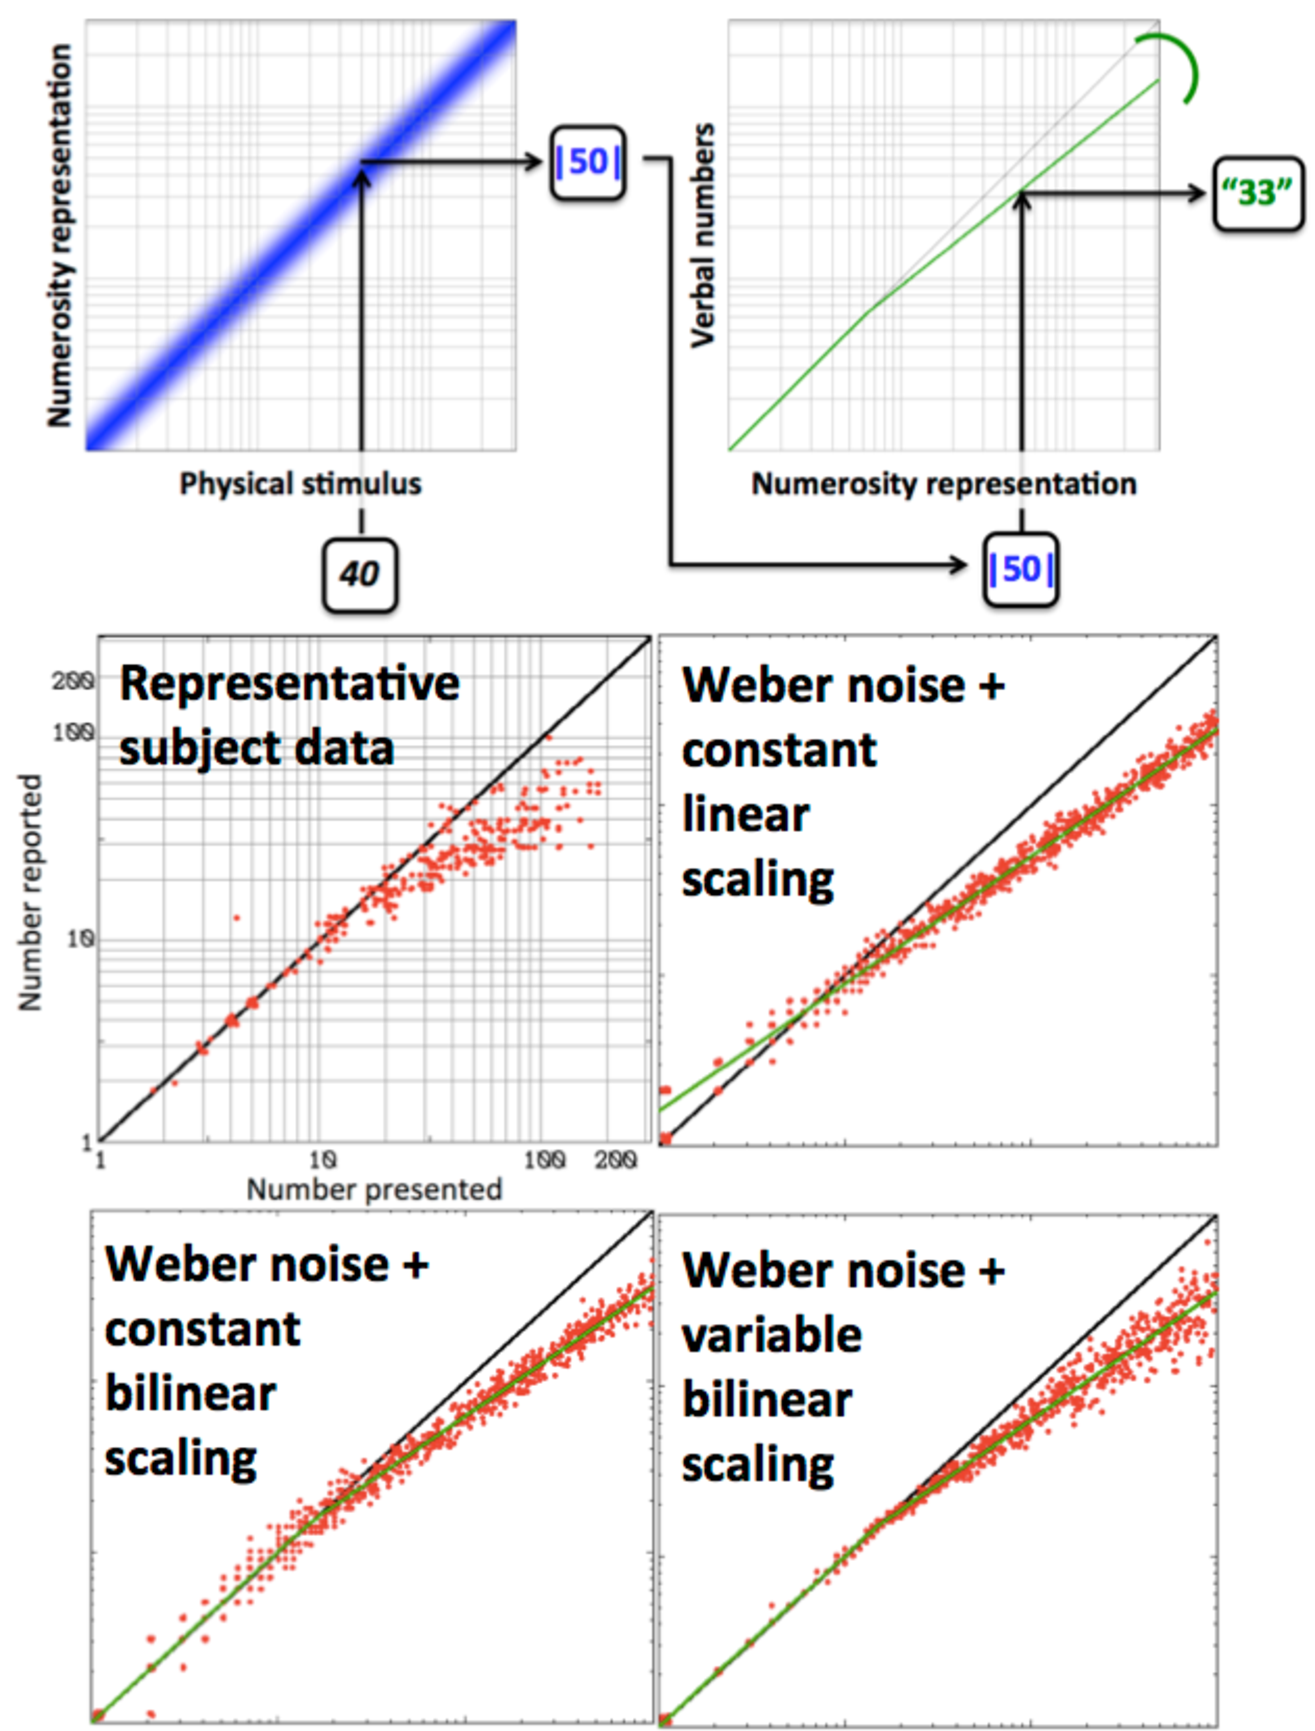
\includegraphics[width=3.3in]{figures/figure-model.pdf}
%\end{center}
\caption{(Top) Our account of the bias and variability in human numerical estimation assumes two two transformations between the physical stimulus and a verbal numerical response.  First, the approximate number system maps the physical stimulus onto a logarithmic magnitude estimate with constant Weber noise.  Second, the magnitude estimates are mapped onto the verbal number; we approximate this mapping as bilinear in log-log space with a variable slope.  (Bottom) Two novel features of this account are necessary to capture the patterns of errors in human estimation data (one representative subject shown): (1) the mapping function must be non-linear in log-log space, otherwise the pattern of veridical calibration for small numbers, and systematic mis-estimation for large numbers will not hold, (2) the slope of the high end of the mapping function must be variable to capture the increasing variability of estimation for larger numbers.} 
\label{figure-model}
\end{figure}

In the absence of training or feedback, adults are notoriously inaccurate estimators (Kaufman, Lord, Resse, \& Volkmann, 1949; Izard \& Dehaene, 2008; Minturn \& Reese, 1951). For the purposes of the present project, we are interested in two attributes of this inaccuracy: variability and bias. 

First, consider the variability of estimates. The degree of variability in estimates increases in proportion to the magnitude of the stimulus being estimated, such that the coefficient of variation (the ratio of the standard deviation of estimates for a given magnitude to the mean estimate of that magnitude) remains constant as magnitude increases (e.g., Whalen et al., 1999). Because variability in estimation behavior scales up with magnitude, estimates are typically said to demonstrate the property of scalar variability. 

\begin{figure}[ht]
\centering
%\begin{center}
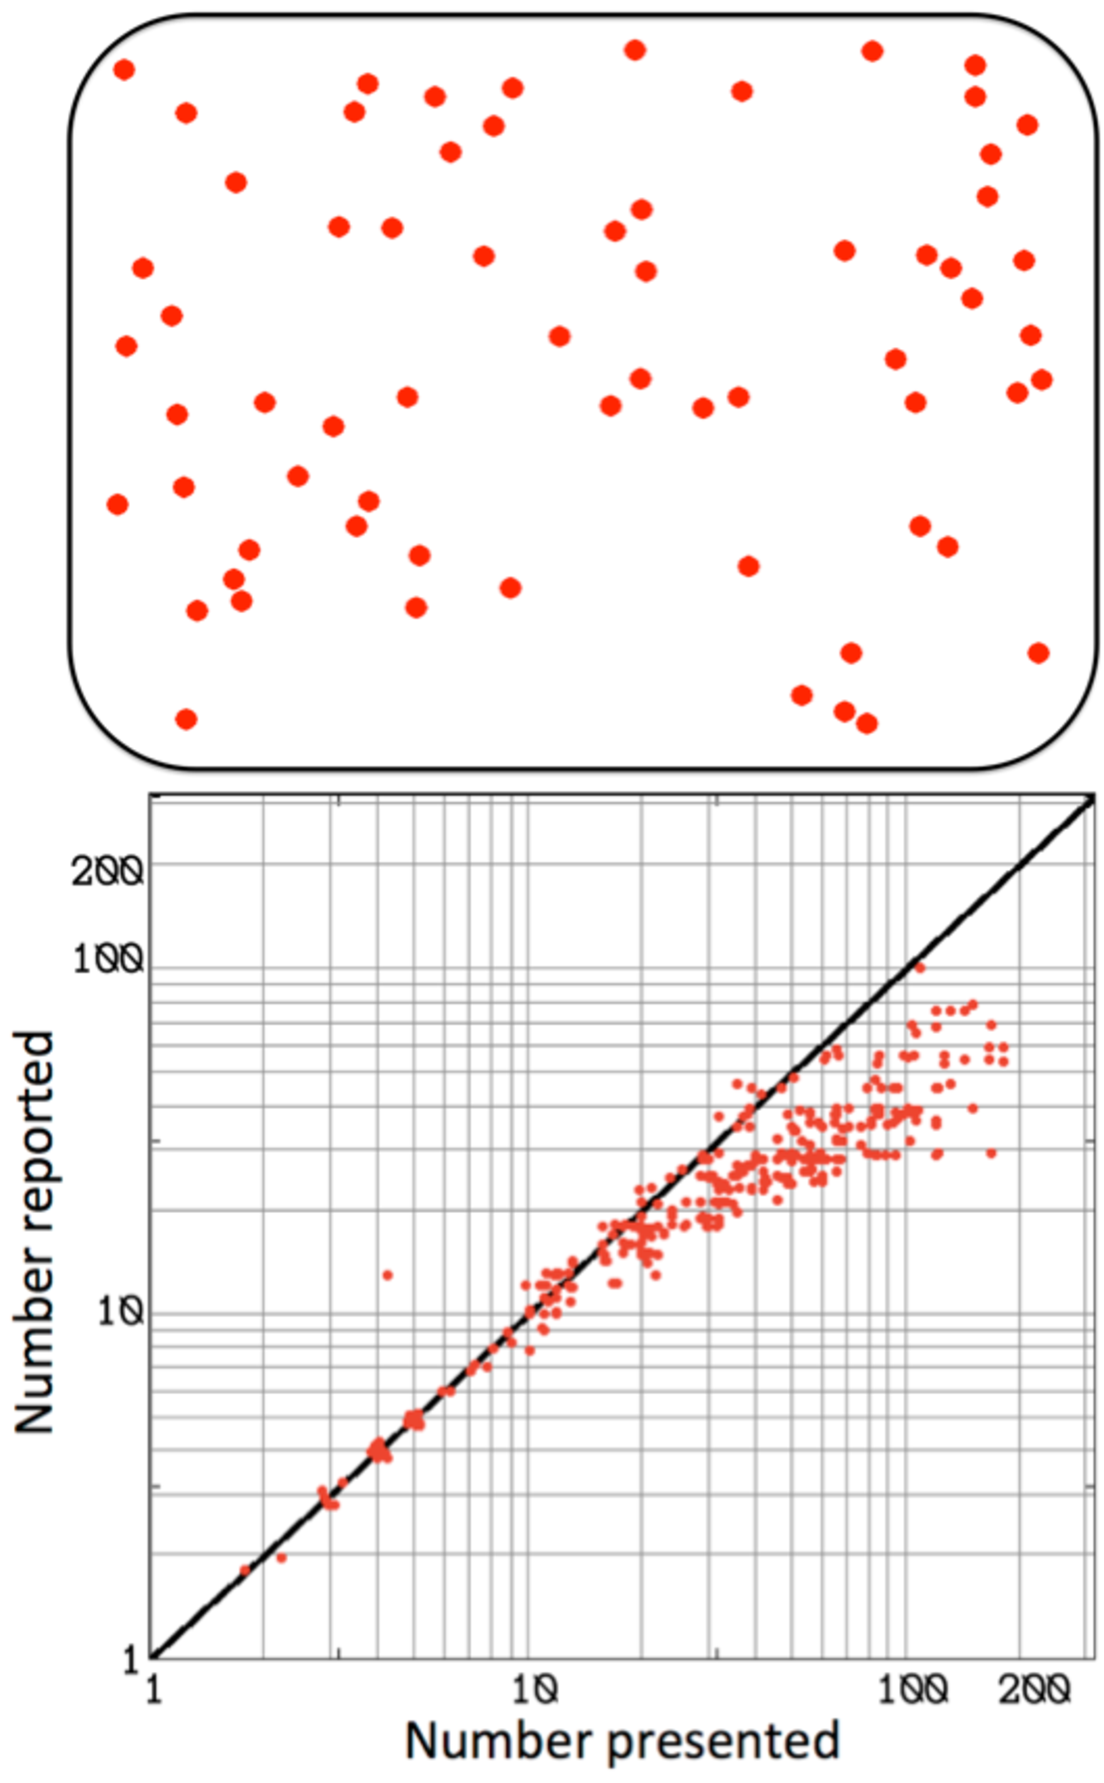
\includegraphics[width=2.5in]{figures/figure-paradigm.pdf}
%\end{center}
\caption{(Top) Participants saw 300 trials in which an array of $n$ dots were briefly presented with the number of dots chosen according to a geometric distribution.  Then participants made a guess as to the number of dots presented.  (Bottom) A representative subject's data over all 300 trials with number presented (log scale) on the x-axis and number reported (log scale) on the y-axis.  We investigate the sources of bias and variability evident in these patterns of mis-estimation.} 
\label{figure-paradigm}
\end{figure}

\begin{figure}[ht]
\centering
%\begin{center}
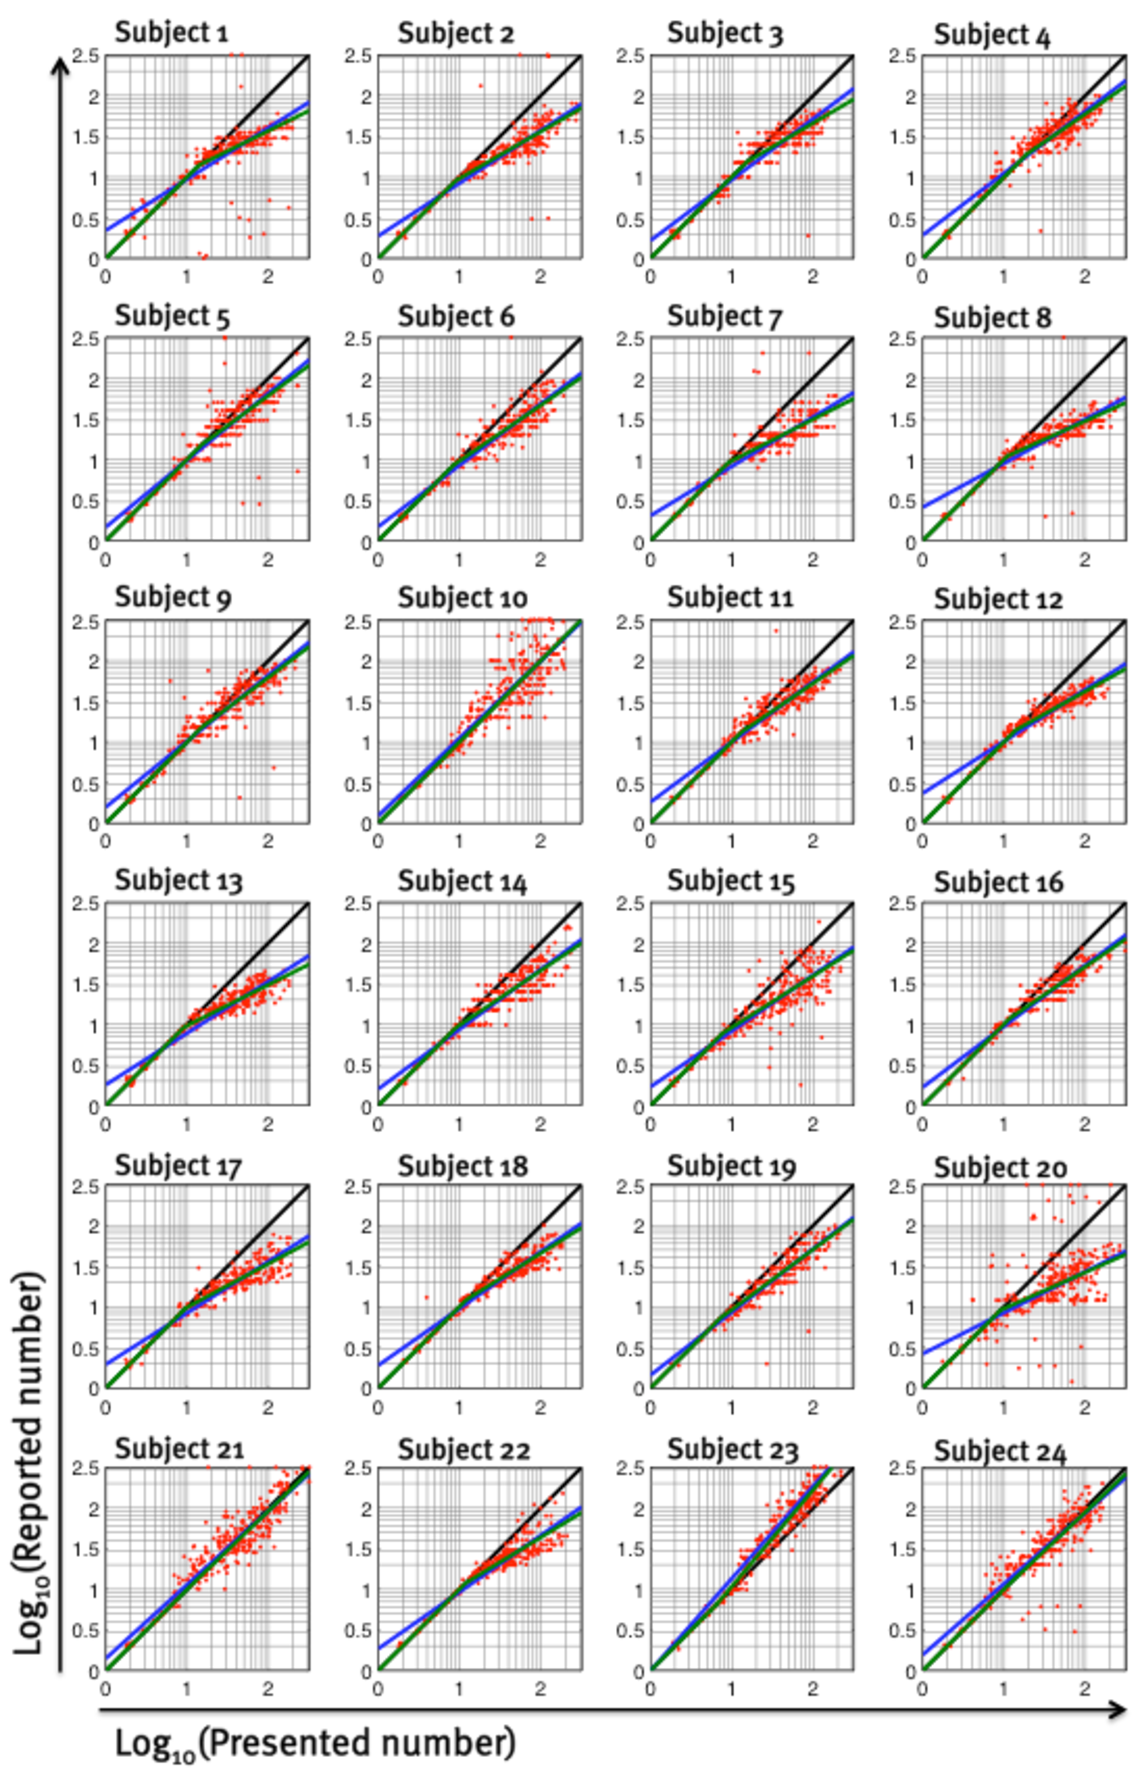
\includegraphics[width=3.4in]{figures/figure-subjects.pdf}
%\end{center}
\caption{Individual subject estimation data.  Some of our conclusions may be seen in the raw data alone: (1) Variability in log-log space increases with numerosity.  (2) Systematic mis-estimation occurs for larger, but not smaller, numbers.  (3) Individual subjects have relatively stable idiosyncratic mis-estimation biases.} 
\label{figure-subjects}
\end{figure}

Scalar variability is thought to arise from Weber noise in the ANS: ANS representations are ratio-dependent, and therefore error in its representation of number also scales with number. For example, it is equally easy to tell the difference between 5 dots and 10 dots as it is to tell the difference between 500 dots and 1000 dots using the ANS. Because both nonverbal ANS tasks and verbal estimation tasks demonstrate scalar variability, many have concluded that scalar variability in estimation arises because the underlying (ANS) perceptual representations of the magnitudes being estimated exhibits weber noise. The assumption that estimation variability indexes variability in ANS representations of magnitude is robust (Dehaene \& Marques, 2002; Izard \& Dehaene, 2008; Le Corre \& Carey, 2007; Negen \& Sarnecka, 2010; Siegler \& Opfer, 2003) and relatively uncontroversial. 

As noted above, it is abundantly clear from the past literature that much of the variability found in estimation arises from variability in the ANS representations that support estimates. However, in the present paper, we ask whether all of the variability in estimation performance is explained by weber noise, or, alternatively, whether the mapping function that connects the verbal and nonverbal number system also contributes variability to estimation performance. One reason to believe that variability and bias may arise in part from the mapping function between number language and the ANS is that feedback (e.g., showing a participant an example) reduces estimation variability in both children and adults (Barth, Starr, \& Sullivan, 2009; Krueger, 1984; Izard \& Dehaene, 2008; Lipton \& Spelke, 2005) � a finding that one might not expect if variability arose entirely from the ANS. However, the degree to which estimation variability stems from the word-to-number mapping function remains untested.

Next, consider estimation bias. One frequent finding in the estimation literature is that estimates tend to be biased (e.g., systematically too high or too low), and bias in estimation performance tends to increase over the course of an experiment. For example, adults often underestimate magnitudes from the very first trial of an estimation experiment, and this bias towards underestimation persists and is amplified over the course of the experiment (Krueger, 1982). In fact, even when the degree and direction of estimation error made early in an experiment is experimentally manipulated, bias introduced in the first few trials endures throughout the duration of the entire estimation experiment (Barth et al., 2009; Izard \& Dehaene, 2008; Krueger, 1984; Lipton \& Spelke, 2005; Shuman, unpublished thesis; Sullivan \& Barner, 2012; Sullivan, Juhasz, Slattery, \& Barth, 2011). This influence of miscalibration is often described as stemming from changes to the number-to-magnitude mapping function. However, the nature of this change in the mapping function is still relatively unstudied. To what extent do previous estimates inform subsequent estimates? Why does the degree of estimation bias change during an estimation task?

In the present study, we test which factors influence errors in estimation performance, with a special focus on the variability and bias found in individual participants� estimates. 

\begin{figure}[ht]
%\centering
%\begin{center}
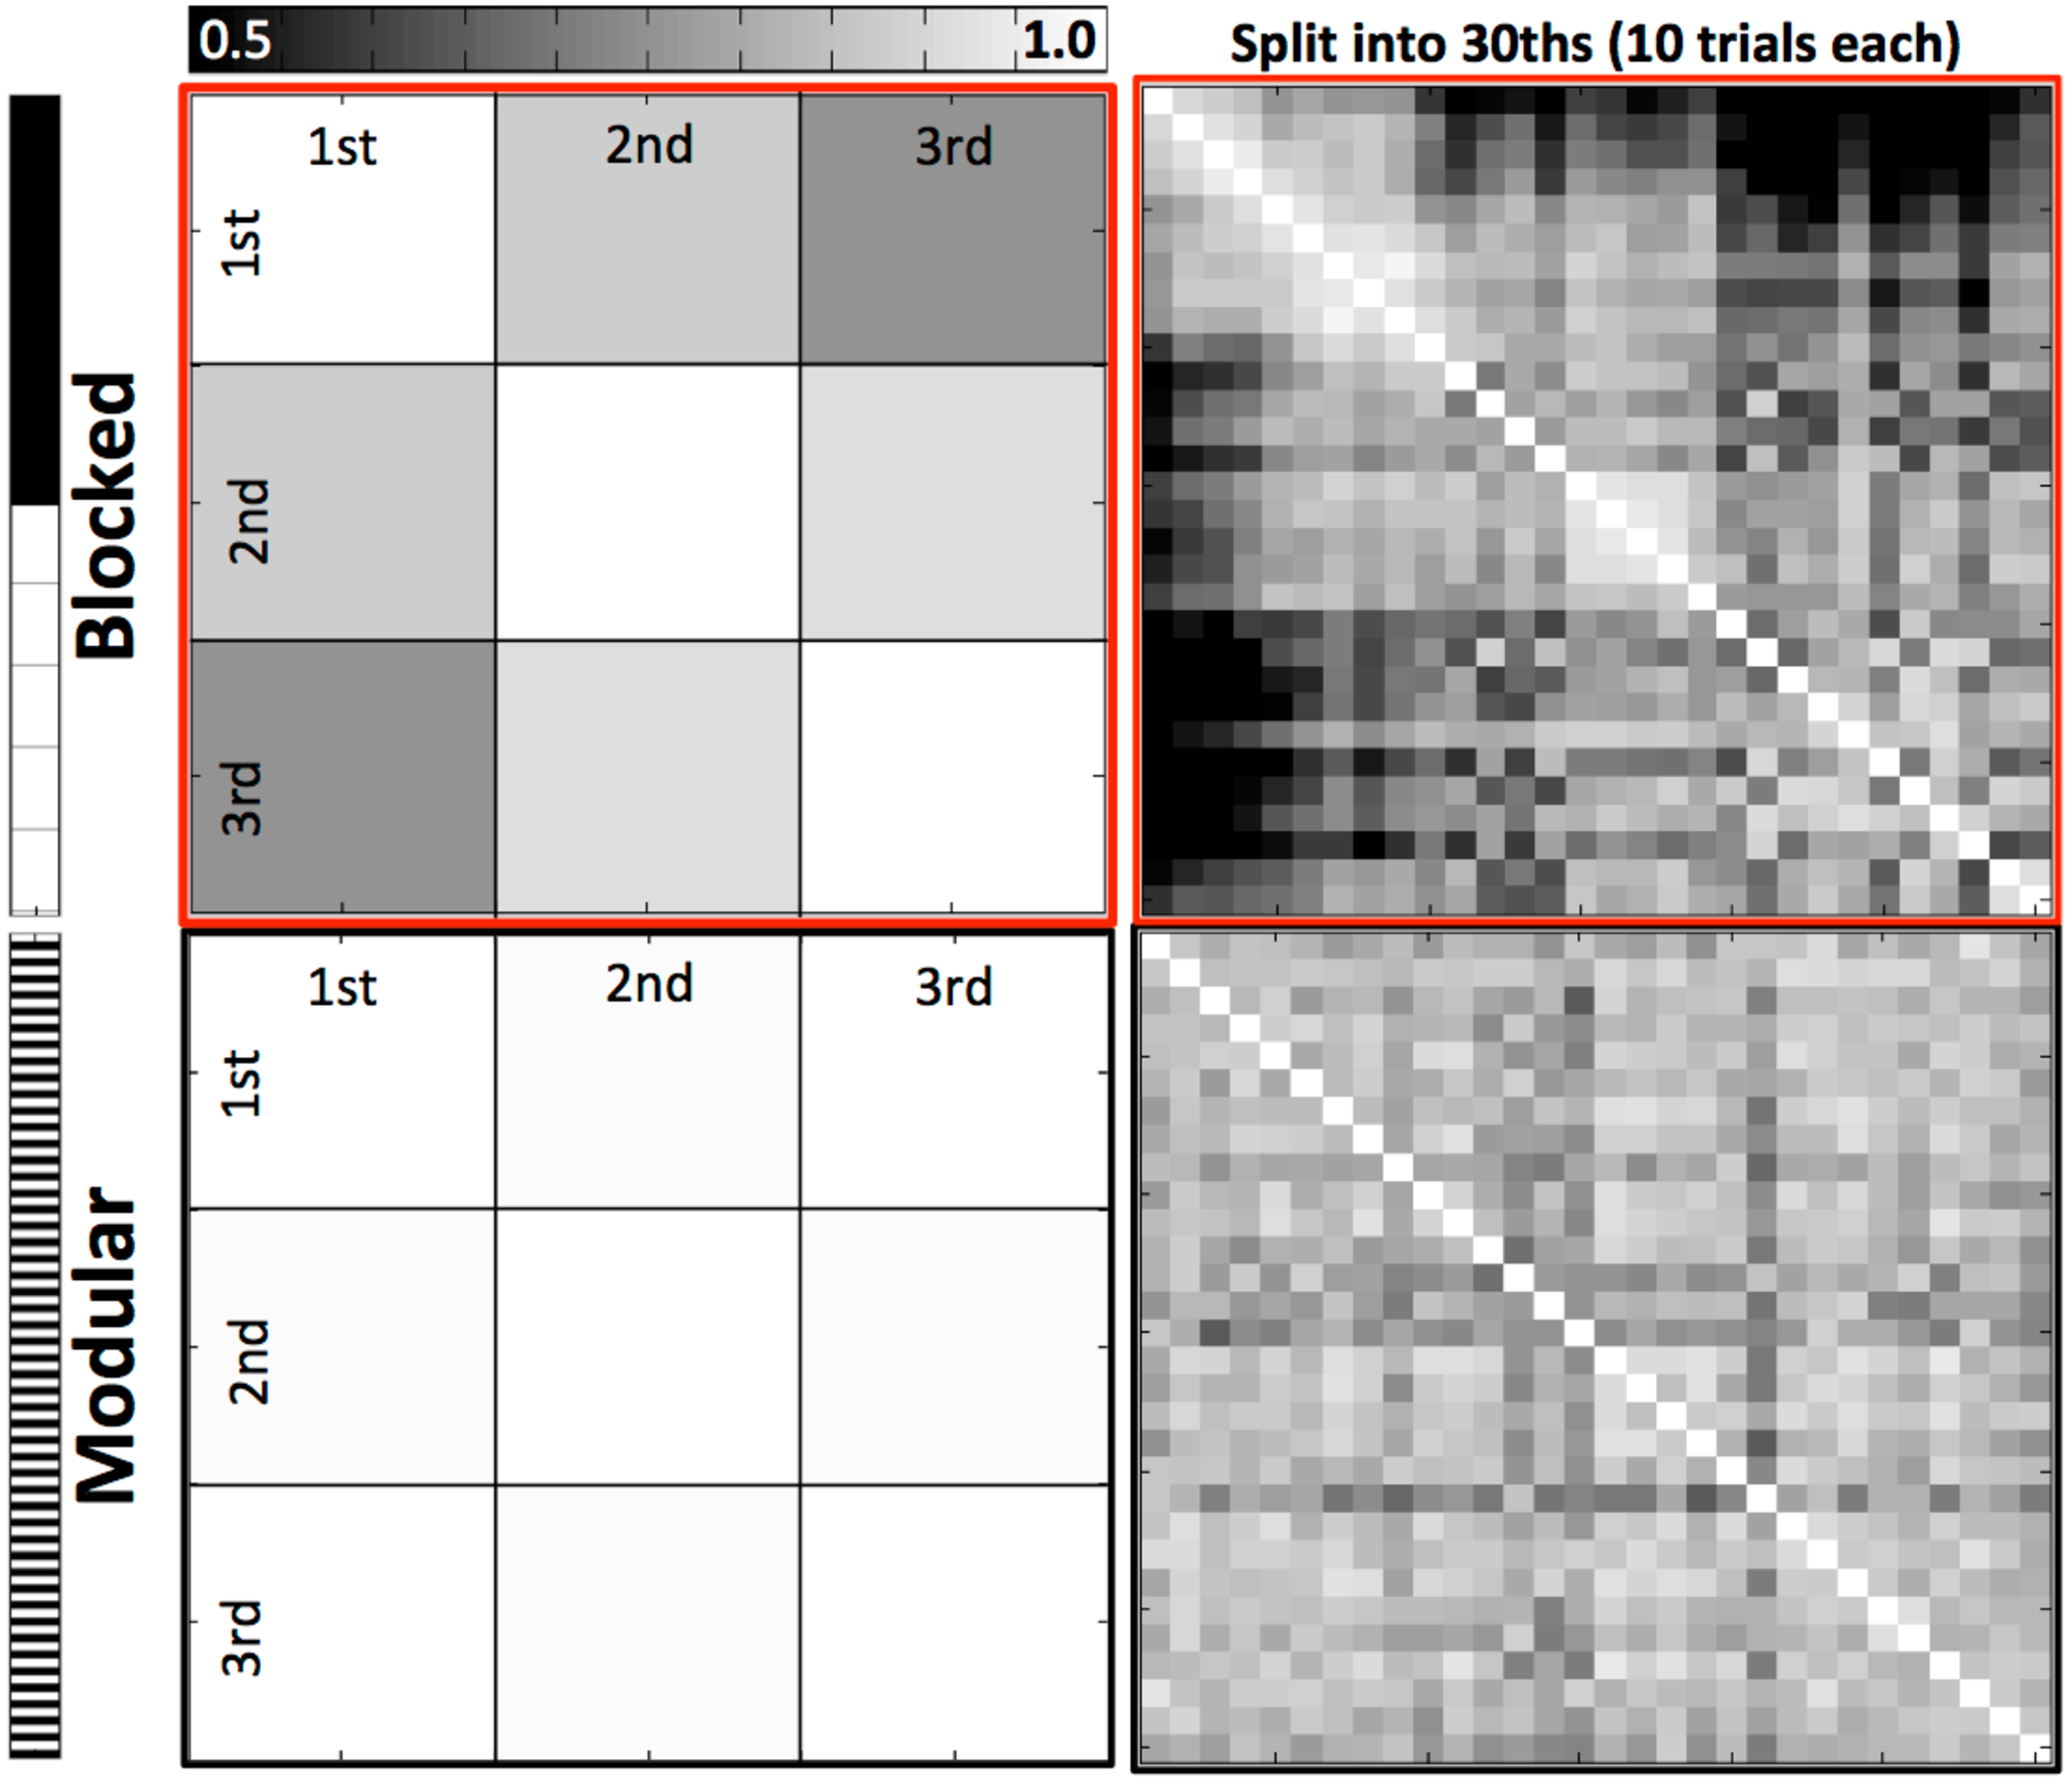
\includegraphics[width=3in]{figures/figure-blocked.pdf}
%\end{center}
\caption{We assess whether variability arises from a slow drift in the mapping function over time by estimating the slope of a bi-linear mapping function for different subsets of the 300 trials for each subject.  For instance, if we split the 300 trials into thirds (left half), then each third contains 100 trials, if we split into thirtieths (right half) then each thirtieth contains 10 trials.  A blocked split (top half) corresponds to taking consecutive portions of the 300 trials: e.g., the first 3rd contains trials 1 through 100, the second 3rd contains trials 101 through 200, the third 3rd contains trials 201 through 300. A modular split (bottom half), corresponds to taking every $n$th trial, such that the full range of the experimental session is represented in each subset: e.g., the first 3rd contains trials 1, 4, 7, 10, ... 298, the second 3rd contains trials 2, 5, 8, 11, ..., 299, and the third 3rd contains trials 3, 6, 9, 12, ..., 300.  We compute the across-subject correlation of slope estimates taken from each subset of trials.  Darker colors indicate lower correlations, brighter colors indicate larger correlations.  Several observations in these heat maps are indicative of a gradual drift in slopes over time within a given subject.  (1) Modular splits yield higher across-subject correlations than blocked splits, suggesting that the blocked splits are subject to additional variability due to a gradual change that modular splits avoid.  (2) Blocked splits show decreasing correlations as a function of distance: correlations further from the diagonal are lower -- the correlation between the first and second third is higher than the correlation between the 1st and 3rd third -- indicating that the correlations are slopes are changing slowly over time.} 
\label{figure-blocked}
\end{figure}

\section{How do people estimate the number of dots?}

We propose that the patterns of bias and variability in human estimation data arises from two transformations between the physical stimulus and a verbal numerical response (see Figure \red{figure-model}): mapping from physical number to approximate magnitudes, and then mapping those magnitudes onto verbal numbers.  

First, the physical stimulus is represented by the approximate number system via a  logarithmic mapping (refs!!) with constant logarithmic noise (i.e. a constant Weber fraction; refs!!).  This internal magnitude representation can be measured directly when people perform numerosity discrimination tasks in which they assess, for instance, which of two arrays has fewer items (!!).  Second, the internal magnitude estimates are mapped onto the verbal number line via a mapping function that is not linear in log-log space (which we approximate as bilinear in log-log space).  Critically, we believe that the slope of the higher portion of this mapping function is variable over time.   

When undertaking an explicit estimation task, these internal magnitude estimates must be mapped on to the verbal number line, and this mapping introduces systematic bias, and additional variability.  Particularly, it is this mapping that introduces systematic underestimation, the magnitude of which scales with numerosity (!!) and can be quickly recalibrated, even with one trial (Dehaene !!).  We propose that because participants have uncertainty in this mapping, the mapping varies over time, thus introducing additional variability in estimation tasks that increases with numerosity.  

For our analyses, we consider this mapping to be bilinear in log-log space: it is veridical (falling on the identity line) for small quantities, but then tends to underestimate for higher numbers.  We do not believe that people actually use a bilinear mapping function -- we suspect that they use a non-parametric function that is constrained to be smooth and monotonically increasing -- however, our data do not offer the resolution necessary to assess whether indeed such a more sophisticated mapping function is used, and for our purposes, approximating this function as bilinear makes our results and analyses easier to describe.

SHOULD BACK OFF FROM THIS: CUT IT ALTOGETHER? Together, this account offers a means to reconcile previous disagreements in the literature on the approximate number system and numerical estimation.  First, while the coefficient of variation (Weber fraction) is constant for the approximate number system, the coefficient of variation in estimates tends to increase with numerosity, suggesting a non-constant Weber fraction.  Our account can reconcile these positions by showing that the coefficient of variation in estimation increases due to variability in the mapping function over time, while discrimination tasks circumvent this mapping by making direct magnitude comparisons.  Second, there is some disagreement as to whether there is a stable (consistent across the numerosity scale) mapping of magnitudes on to verbal numbers (!!), our account can resolve this tension because while there appears to be a mapping of magnitudes to numbers that is consistent across the range of magnitudes at any one point in time, this mapping is not stable over time, yielding inconsistent behavior over trials.

\begin{figure}[ht]
%\centering
%\begin{center}
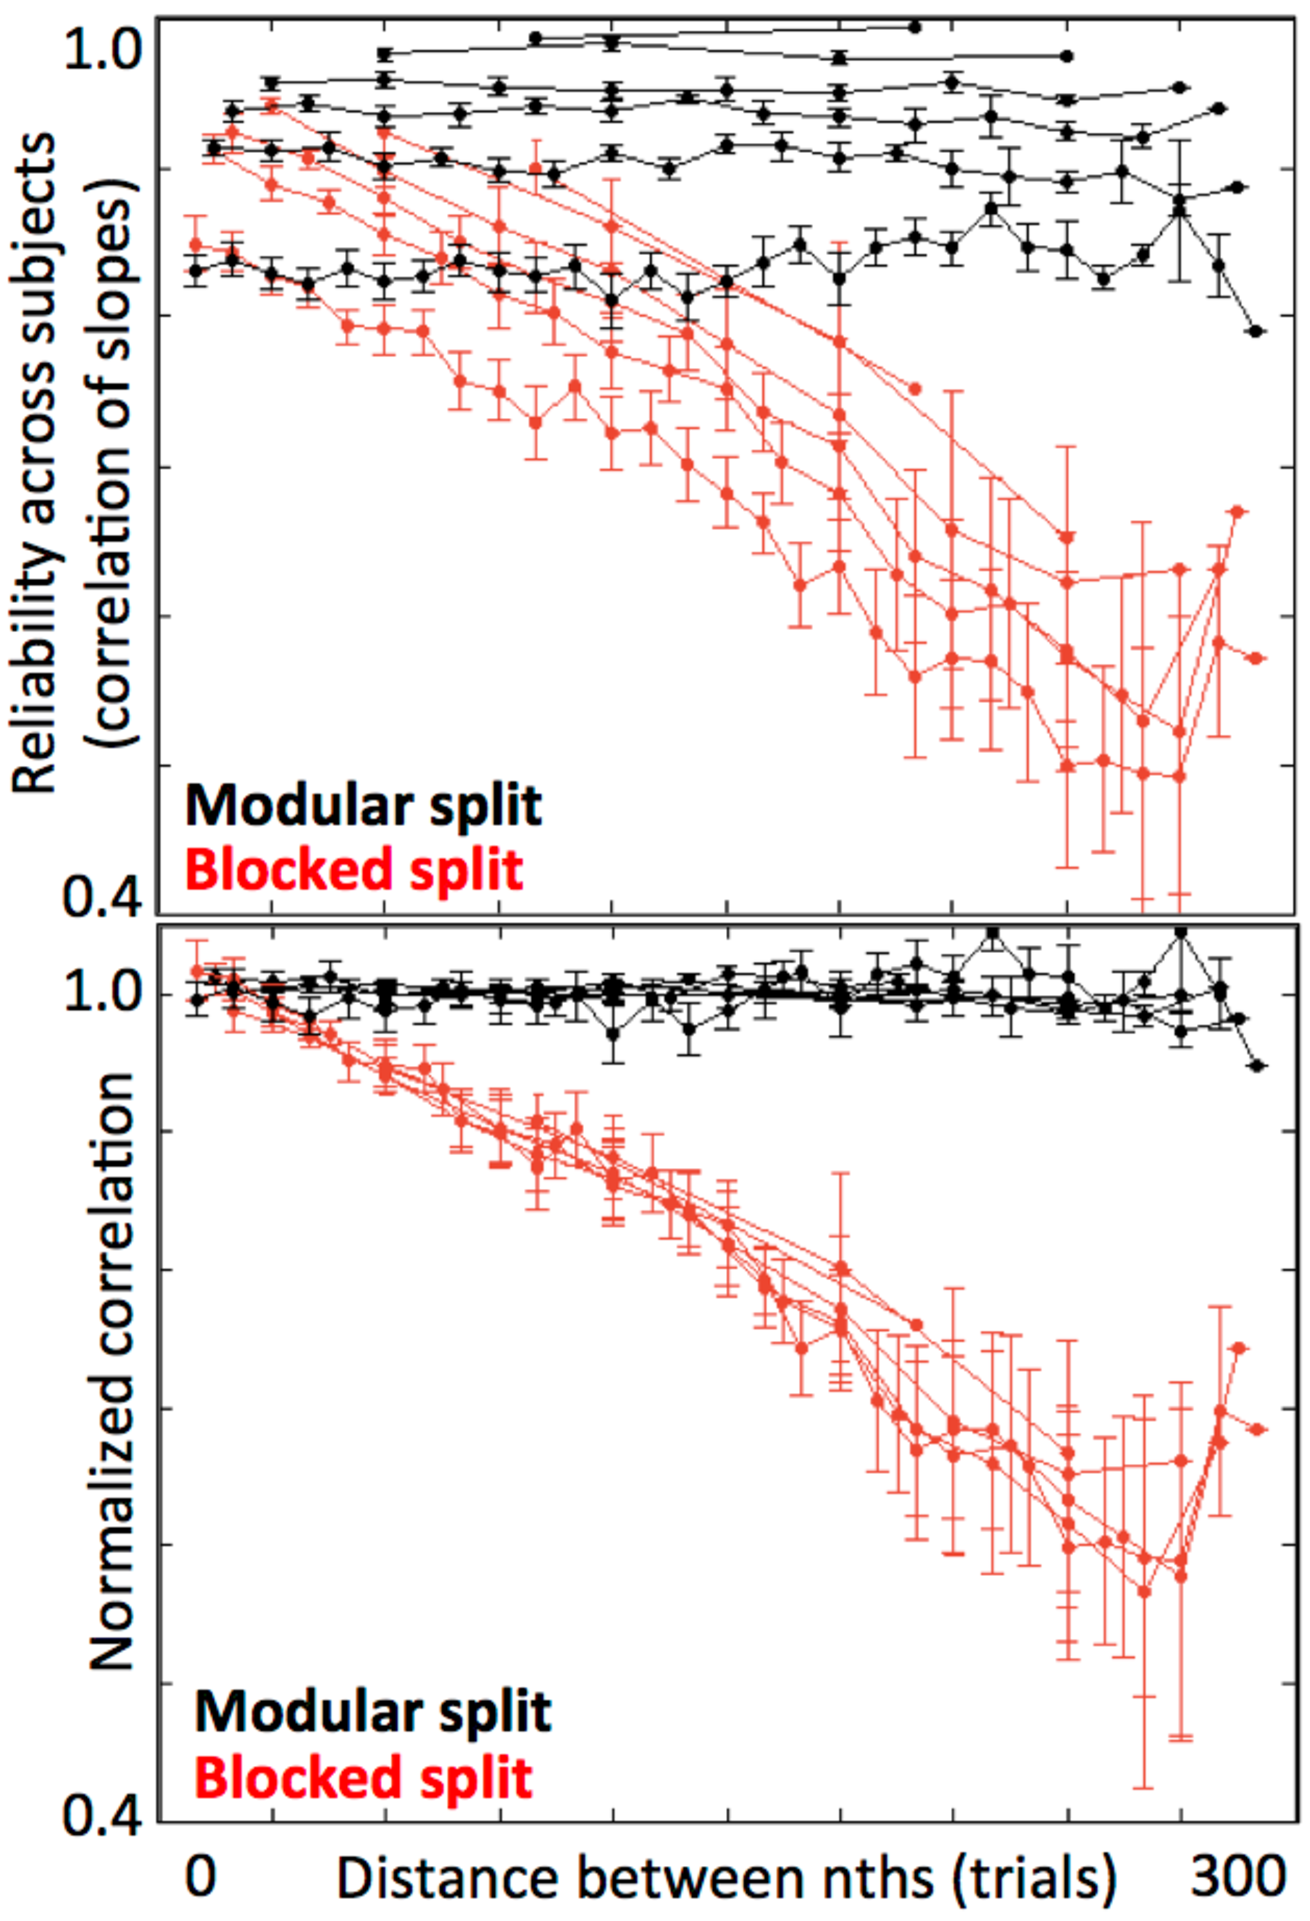
\includegraphics[width=3in]{figures/figure-correlations.pdf}
%\end{center}
\caption{(Top) We can assess the average across-subject correlation in slope estimates as a function of distance between blocks for different splits of the data.  A blocked split of the data into thirds yields a two measures of the slope-correlation at an average distance of 100 trials (1st to 2nd block and 2nd to 3rd block) and one measure of the correlation at a distance of 200 trials (1st to 3rd block).  If we split the data more finely (here going up to 30ths, as seen in figure , we can more finely measure the drop-off of average correlation as a function of distance.  Distance is meaningless for Modular (points in black) splits, but the same analysis can be carried out to measure how much the correlation drops merely as a function of using fewer trials for each slope estimate.  (Bottom) we can normalize both blocked (red) and modular (black) correlations to the average of the modular split correlations to make the decrease in correlation with distance as seen in the red lines comparable across splits with different numbers of trials per subset.  Correlations drop off with distance very slowly, but even when separated by 290 trials, 10-trial estimates of subjects' mapping function slopes show reliabilities well above 0.}
\label{figure-correlations}
\end{figure}

Figure \ref{figure-model} provides an illustration of our model, and shows predictions from reduced classes of this model as compared to one (representative) subject's data.  With only constant Weber noise and a stable linear mapping of magnitudes to numbers, to account for the variability and underestimation seen for larger numbers, we would erroneously predict overestimation and too much variability for small numbers.  Even with a bi-linear mapping, constant Weber-fraction variability would under-predict variability for large numbers and over-predict variability for small numbers.  Only with a variable slope in a bi-linear mapping function can we account for the pattern of miscalibration and increasing variability for large, but not small, numbers.  In the subsequent section we describe analyses that explicitly measure and and test these claims. 

\section{Experiment Methods}

Twenty-four subjects recruited from the UC San Diego psychology department pool participated in an hour-long experiment in which they had to guess the number of dots presented onscreen on each trial (see Figure \ref{figure-paradigm}).  The number of dots shown was sampled from a geometric distribution with a mean of 50, truncated at the low end so that displays had at least two dots.  All the dots in an array were the same size (radius of 10 pixels), presented in red on a white background.  The configuration of dots was randomly generated by drawing locations from a uniform distribution over the full display area (1024x768 pixels) with the constraint that the dots did not overlap.  On each trial the array of dots was presented for 250 msec, and then subjects were prompted to type in their guess as to how many dots were in the array.  Subjects were then asked to type in a second guess about the number of dots in the array.  (Our analyses throughout the paper focus on the first of the two guesses, but our conclusions hold if we consider the second guess alone, or the average of the two).  Figure \ref{figure-paradigm} also shows one representative subject's data from all 300 trials.

\section{Results}


The responses of all 24 participants for all 300 trials in our experiment are shown in Figure \ref{figure-subjects} on log-log coordinates.  Several features of the data immediately jump out. First, estimate variability goes up as a function of number.  Since this is an increase in variability in log-log space, it is not consistent with a constant coefficient of variation (a constant Weber fraction) which predicts that variability would be constant in log-log space.  Second, while people are well calibrated for small numbers, there is a tendency to underestimate large numbers: most subjects underestimate, but some subjects show fairly reliable overestimation or veridical average calibration.  Third, individual differences in under- or over- estimation appear to be quite reliable.  These superficial features are consistent with our account of a variable mapping function, and we will refine these results in specific analyses below.

\subsection{Is magnitude-to-number mapping bilinear?}

We propose that the mapping function is not linear in log log space, but bends such that low numbers are mapped more or less correctly onto numbers, but large numbers show a systematic deviation from the identity line.  While we do not believe that the true mapping function that people entertain is strictly bilinear, we do believe that it is not simply linear in log-log space.  We can show that a bilinear function that is veridical (falls on the identity line) up to some critical number ($c$), and then deviates from the identity line with some log-log slope of $s$ can account for data of individual subjects much better than a simple line with an intercept ($a$) and a slope ($b$).  Since these models both have two parameters, we can simply compare the $R^2$ values of individual subjects.  Although the average $R^2$ values are similar (0.79, vs 0.81), bilinear fits better describe the data for 20 of 24 subjects (binomial test: $p=0.0015$), see Figure \ref{figure-subjects}.  

This piecewise-linear mapping function could indicate a number of possible processes.  Perhaps small numbers (less than about 10 -- the average point of departure from veridical mapping across subjects) are not part of the mapping between the approximate number system and words, and are instead remembered separately.  Another possibility is that the mapping function is constrained by previous data clearly disambiguating the numerosity/numbers correspondence, and lower numbers have more data, and thus fall on the identity line, while higher numbers are constrained only by a requirement for smoothness and monotonicity.  We slightly favor the second alternative, only because the cut-off point between accurate and miscalibrated mapping  does not seem to correspond to other cut-offs previously postulated to distinguish between qualitatively different numerosity processes (such as subtilizing and approximate magnitude -- typically described as a cutoff between 4 and 6; cite!!).

\subsection{Is there variability in the mapping function over time?}

We argue that some of the increase in variability of estimates with increasing number arises from variability of the {\em mapping function} over trials, rather than simple misperception of the approximate magnitude of an individual array.  In this section we argue for this view because the internal mapping function drifts slowly over the course of many trials, and we can measure its variation over the course of an experimental session.

To measure any drift in the mapping function over time, we estimate the mapping function (particularly the slope of the higher bilinear portion) in individual subjects in different subsets of the experimental trials.  We can then assess the across-subject correlation between different subsets of trials, to see whether variation of slopes across subjects is less reliable when considering mapping function estimates obtained from trials separated further in time.

First we assess the split-half reliability of slope estimates when we split the trials in half using two methods.  {\em Blocked} split-half divides the 300 trials into the first half (1-150) as subset 1, and  the second half (151-300) as subset 2; thus, for blocked splits, the trials in a given subset are contiguous, and the different subsets come from different portions of the experiment (separated by an average of 150 trials).  {\em Modular} split-half divides the 300 trials into odd trials (1, 3, 5, ..., 299) as subset 1, and even trials (2, 4, 6, ..., 300) as subset 2; thus, for modular splits, the trials in a given subset are taken from the full range of the experiment.  If the slopes we estimate for the mapping function drift over time, we expect that Blocked splits should yield a lower split-half across-subject reliability score than Modular splits, because the Blocked splits are taken from different points in time, and would reflect different stats of drift of the mapping function, while Modular splits would not.  Indeed, this is exactly what we find: the Blocked split-half reliability of slope estimates is $r=0.83$ and the Modular split-half reliability is $r=0.97$: while both are significant, Blocked is significantly lower ($z=-2.74$, $p=0.0061$). This is our first indication that the slope of the magnitude-number mapping function is not stable within individuals over the experimental session.

To more precisely measure the drift of the mapping function over time, we generalize the Blocked vs. Modular split-half analysis to Blocked vs. Modular split-$n$ths for $n=\{3, 5, 10, 15, 20, 30\}$ (e.g., split-30th divide our 300 trials into 30 subsets, each one comprising 10 trials, for instance, the 5th Blocked split-30th subset will contain trials 41-50, while the 5th Modular split-30th subset will contain the 10 trials: 5, 35, 65, 95, 125, 155, 185, 215, 245, 275).  By obtaining split-$n$th reliability for Blocked subsets taken from different portions of the experimental session, we can assess how the reliability of the number-mapping slope decreases as a function of time.  

We calculate the across-subject slope reliability across different subsets (represented as a matrix in Figure \ref{figure-blocked}), the Blocked split-$n$th reliability between subset 1 and subset 2 measures the across-subject correlation of slopes estimated from two adjacent periods of time in the session which are on average separated by $300/n$ trials.  In general if we calculate the correlation between subset $i$ and subset $i+k$ from a Blocked split-$n$th analysis, those subsets are separated by $300*k/n$ trials.  Thus, if slopes are gradually drifting over the course of the experimental session, we would expect across-subject reliability of slope estimates to decrease with $k$ -- the separation between Blocked subsets.  Nothing of this sort should happen for Modular subsets which contain overlapping trials intermixed over the whole session.  

Figure \ref{figure-correlations}(top) shows the split-$n$th reliability for Blocked (red) and Modular (black) subsets as a function of their separation ($k$).  For instance, we estimate the average Blocked split-$10$th correlation at a separation of $k=2$ as the average of the across-subject correlations taken between the 8 subset comparisons separated by 2: subset 1 and subset 3, subset 2 and subset 4, ... subset 8 and subset 10.  This average would appear at $x=300/n*k=300/10*2=60$.  Several features are apparent from the changes in slope reliability across subsets separated by more time: (1) when we split into more subsets both Modular and Blocked correlations drop, since each subset necessarily contains fewer trials to estimate the slope; (2) as expected, only Blocked correlations decrease as a function of distance between subsets.  To more clearly display the decrease in reliabilities as a function of subset distance, while factoring out the reduced reliability due to smaller trial-counts within each subset, by normalizing reliabilities by dividing them by the average reliability seen across Modular splits.  This yields Figure \ref{figure-correlations}(bottom), which shows the slow decrease in reliabilities over the 300 trials.  

A linear regression on the raw correlations in the Blocked split-$n$ths as a function of separation (measured in trials) is significantly negative (95\% confidence interval on the slope: $(-0.0015, -0.0012)$ change in correlation per trial,  $F(1,22)=358$, $p<0.001$).  Despite this highly significant decrease, it is very slow over the course of the session, and even mapping function slope estimates based on 10 trials separated by 290 trials show significant across-subject reliability ($r=0.57$; $t(22)=3.254$, $p=0.002$).  

Together, these results indicate that subjects' mappings of magnitudes onto verbal numbers drift slowly over time. 

!! include?? experiments not reported here suggest that this drift arises from uncertainty in the magnitude-number mapping, since 250 trials with feedback (veridical, or otherwise), induces a particular calibration which remains quite stable for as long as 250 trials after feedback stops.

%\subsection{Why is there drift?  Rate of drift consistent with autoregressive process.}
%
%The last question we ask is: given that there is drift over time, is it the case that subjects really have their own idiosyncratic mapping biases, or are we simply measuring them at a particular point in time.  In other words, if we wait long enough, will the random drift cause our participants to be indistinguishable from one another in the long run?  We can ask this question by assessing whether the drift rate is constant.
%
%If (as we suspect) participants do show drift, but this drift is restricted to the range of their own bias and uncertainty, then we should see a mean-reverting drift: one that tends to hang around the same slope value.  If this is the case, then the apparent rate of drift will decrease over time: a measure of the drift between block 1 and block 2 will be bigger than 1/10th of the drift that occurred between block 1 and block 11.  In contrast, if the drift is not mean reverting, then these drift rates should be constant.  
%
%The drift will be mean-reverting even if all subjects have a single bias... how do we figure out if they are stable?
%

\section{Conclusions}

We argue that people map !!


\vspace{2mm}

\begin{small}
\noindent {\bf Acknowledgments:} EV was supported by the Intelligence Advanced Research Projects Activity (IARPA) via Department of the Interior (DOI) contract D10PC20023. The U.S. Government is authorized to reproduce and distribute reprints for Governmental purposes notwithstanding any copyright annotation thereon. The views and conclusions contained herein are those of the authors and should not be interpreted as necessarily representing the official policies or endorsements, either expressed or implied, of IARPA, DOI, or the U.S. Government. 

\section{References}
\begin{hangparas}{.125in}{1}
\setlength{\parskip}{0em}

Barth, H., Starr, A., & Sullivan, J. (2009). Children�s mappings of large number words to numerosities. Cognitive Development, 24, 248-264.

Carey, S. (2009). The Origin of Concepts. Oxford University Press: New York. 

Dehaene, S. (1997). The Number Sense: How the Mind Creates Mathematics. Oxford University Press: New York.

Dehaene, S., & Marques, J. (2002). Cognitive euroscience: Scalar variability in price estimation and the cognitive consequences of switching to the euro. The Quarterly Journal of Experimental Psychology, 55, 705-731.

Ebersbach, M., Luwel, K., Frick, A., Onghena, P., Verschaffel, L. (2008). The relationship between the shape of the mental number-line and familiarity with numbers in 5- to 9-year old children: Evidence for a segmented linear model. Journal of Experimental Child Psychology, 99, 1-17.

Izard, V., & Dehaene, S. (2008). Calibrating the mental number line. Cognition, 106, 1221-1247.

Kaufman, E., Lord, M., Reese, T., & Volkmann, R. (1949). The discrimination of visual number. The American Journal of Psychology, 62, 498-525.

Krueger, L. (1982). Single judgments of numerosity. Perception and Psychophysics, 31,  175-182.

Krueger, L. (1984). Perceived numerosity: A comparison of magnitude production, magnitude estimation, and discrimination judgments. Perception and Psychophysics, 35,  536-542.

Le Corre, M., & Carey, S. (2007). One, two, three, four, nothing more: An investigation of the conceptual sources of the verbal counting principles. Cognition, 105, 395-438. 9, 159-172.

Lipton, J., & Spelke, E. (2005). Preschool children�s mapping of number words to nonsymbolic numerosities. Child Development, 76, 978-988.

Minturn, A., & Reese, T. (1951). The effect of differential reinforcement on the discrimination of visual number. Journal of Psychology, 31, 201-231.

Negen, J., & Sarnecka, B. (2010). Analogue magnitudes and knower-levels: Re-visting the variability argument. Proceedings of the 32nd Annual Conference of the Cognitive Science Society, Austin, TX: Cognitive Science Society.

Ramani, G., & Sieger, R. (2011). Reducing the gap in numerical knowledge between low- and middle-income preschoolers. Journal of Applied Developmental Psychology, 32, 146-159.

Shuman, M. (unpublished thesis). Computational characterization of numerosity perception and encoding.

Siegler, R., & Opfer, J. (2003). The development of numerical estimation: Evidence for multiple representations of numerical quantity. Psychological Science, 14, 237-243. 

Siegler, R., & Ramani, G. (2009). Playing linear number board games�but not circular ones�improves low-income preschoolers� numerical understanding. Journal of Educational Psychology, 101, 545-560.

Sullivan, J., & Barner, D. (2012). How are number words mapped to approximate magnitudes? Quarterly Journal of Experimental Psychology, 66, 389-402.

Sullivan, J., Juhasz, B., Slattery, T., & Barth, H. (2011). Adults� number-line estimation strategies: evidence from eye movements. Psychonomic Bulletin and Review, 18, 557-563.

Thompson, C., & Opfer, J. (2010). How 15 hundred is like 15 cherries: Effect of progressive alignment on representational changes in numerical cognition. Child Development, 81, 1768-1786.

Whalen, J., Gallistel, C., & Gelman, R. (1999). Nonverbal counting in humans: the psychophysics of number representation. Psychological Science, 10, 130-137.











\end{hangparas} 
\end{small}



\end{document}